\documentclass{article}
\usepackage{graphicx}
\usepackage{subcaption}
\usepackage{amssymb, amsmath, amsthm}
\title{Homework 4 : Bayesian Networks and kNN}
\author{Elnur Gasanov : 163411}
\pagestyle{plain}

\newcommand{\mw}[0]{\bold{w}}
\newcommand{\mm}[0]{\bold{m}}
\newcommand{\mx}[0]{\bold{x}}
\newcommand{\mS}[0]{\bold{S}}

\parindent=0.0mm

\begin{document}
\maketitle

\section{Fisher's linear discriminant}

We start with 

$$
J(\mw) = \frac{(m_1 - m_2)^2}{s_1^2 + s_2^2}
$$

We separately analyse the nominator and the denominator of the above formula.

$$
(m_1 - m_2)^2 = (m_1 - m_2)^\intercal (m_1 - m_2) = \mw^\intercal (\mm_1-\mm_2) (\mm_1 - \mm_2)^\intercal \mw = \mw^\intercal \mS_B \mw.
$$

$$
s_1^2 + s_2^2 = \sum\limits_{n\in \mathcal{C}_1} (y_n - m_1)^2 + \sum\limits_{n\in \mathcal{C}_2} (y_n - m_2)^2 = 
$$

$$
\sum\limits_{n\in \mathcal{C}_1} (y_n - m_1)^\intercal (y_n - m_1) + \sum\limits_{n\in \mathcal{C}_2} (y_n - m_2)^\intercal (y_n - m_2) = 
$$

$$
\sum\limits_{n\in \mathcal{C}_1} \mw^\intercal (\mx_n - \mm_1) (\mx_n - \mm_1)^\intercal \mw + \sum\limits_{n\in \mathcal{C}_2} \mw^\intercal (\mx_n - \mm_2) (\mx_n - \mm_2)^\intercal \mw = 
$$
$$
\mw^\intercal \left( \sum\limits_{n\in \mathcal{C}_1} (\mx_n - \mm_1) (\mx_n - \mm_1)^\intercal + \sum\limits_{n\in \mathcal{C}_2}(\mx_n - \mm_2) (\mx_n - \mm_2)^\intercal \right) \mw = \mw^\intercal \mS_W \mw.
$$

Finally, we get that

$$
\boxed{J(\mw) = \frac{\mw^\intercal \mS_B \mw}{\mw^\intercal \mS_W \mw}}.
$$

\section{Conditional independence}

From the structure of the Bayes Net we get that $p(a, b, c) = p(a) p(b|a) p(c|b)$.

Hence,

$$
p(a, c| b) = \frac{p(a, b, c)}{p(c)} = \frac{p(a) p(b|a) p(c|b)}{p(c)} = p(c|b) \frac{p(a) p(b|a)}{p(c)}{p(c)} = p(c|b) p(a|b)
$$

\section{Bayesian Network}

\subsection{Computing conditional probability}

We will compute some joint probabilities in top-bottom directions (when looking at the net).

$$
p(+u|+i) = \sum\limits_h p(+u| +i, h) p(h) = 0.66
$$
$$
p(+u|-i) =  \sum\limits_h p(+u| -i, h) p(h) = 0.34
$$
$$
p(+t+u) = \sum\limits_i p(+t+u|i) p(i) = \sum\limits_i p(+t|i)p(+u|i) p(i) = 0.4206
$$
$$
p(-t+u) = \sum\limits_i p(-t|i)p(+u|i) p(i) = 0.1434
$$
$$
p(+t-u) = \sum\limits_i p(+t|i)p(-u|i) p(i) = 0.2894
$$
$$
p(-t-u) = 0.1466
$$
$$
p(+e+u) = \sum\limits_t p(+e|+u,t) p(+u,t)= 0.47892
$$
$$
p(+e) = \sum\limits_{u, t} p(+e|u,t) p(u, t) = 0.6676
$$
$$
\boxed{p(+u | +e) = \frac{p(+e,+u)}{p(+e)} \approx 0.717}
$$


\subsection{True/False}

\begin{enumerate}
	\item False. When I is not observed, then the only "tail-to-tail" connection in the path $t \rightarrow i \rightarrow u$ is unblocking.
	\item False. When E is observed, then the only "head-to-head" connection in the path $t \rightarrow e \rightarrow u$ is unblocking.
	\item True. All paths are blocked (there are only one connection in each path)
	\item False. In the path $h \rightarrow u \rightarrow i \rightarrow t \rightarrow e$ all connections are unblocking.
	\item True. All path are blocked. ($h \rightarrow u \rightarrow e$ is blocked, since U is observed; in the path $h \rightarrow u \rightarrow i \rightarrow t \rightarrow e$ connection $uit$ is blocking.
	\item False. E is a descendant of U, connection/path $hui$ is "head-to-head". 
	\item True. Path $h \rightarrow u \rightarrow i$ is blocked, since U is not observed, in the path $h \rightarrow u \rightarrow e \rightarrow t \rightarrow i$ connection $eti$ is blocking.
	\item True. In the path $h \rightarrow u \rightarrow i \rightarrow t$ blocking connection is $hui$, in the path $h \rightarrow u \rightarrow e \rightarrow t$ blocking connection is $uet$.
	\item False. In the path $h \rightarrow u \rightarrow e \rightarrow t$ every connection is unblocking.
	\item False. In the path $h \rightarrow u \rightarrow i \rightarrow t$ every connection is unblocking.
\end{enumerate}

\section{kNN}

A standard algorithm and an adaptive Parzen-Rosenblatt window classifier were implemented. Kernel function $K(x) = 1.01 - x $ was used in the second method. Errors on testing data for both algorithms are presented on graphs below.

\begin{figure*}[t]
    \centering
    \begin{subfigure}[b]{0.5\textwidth}
        \centering
        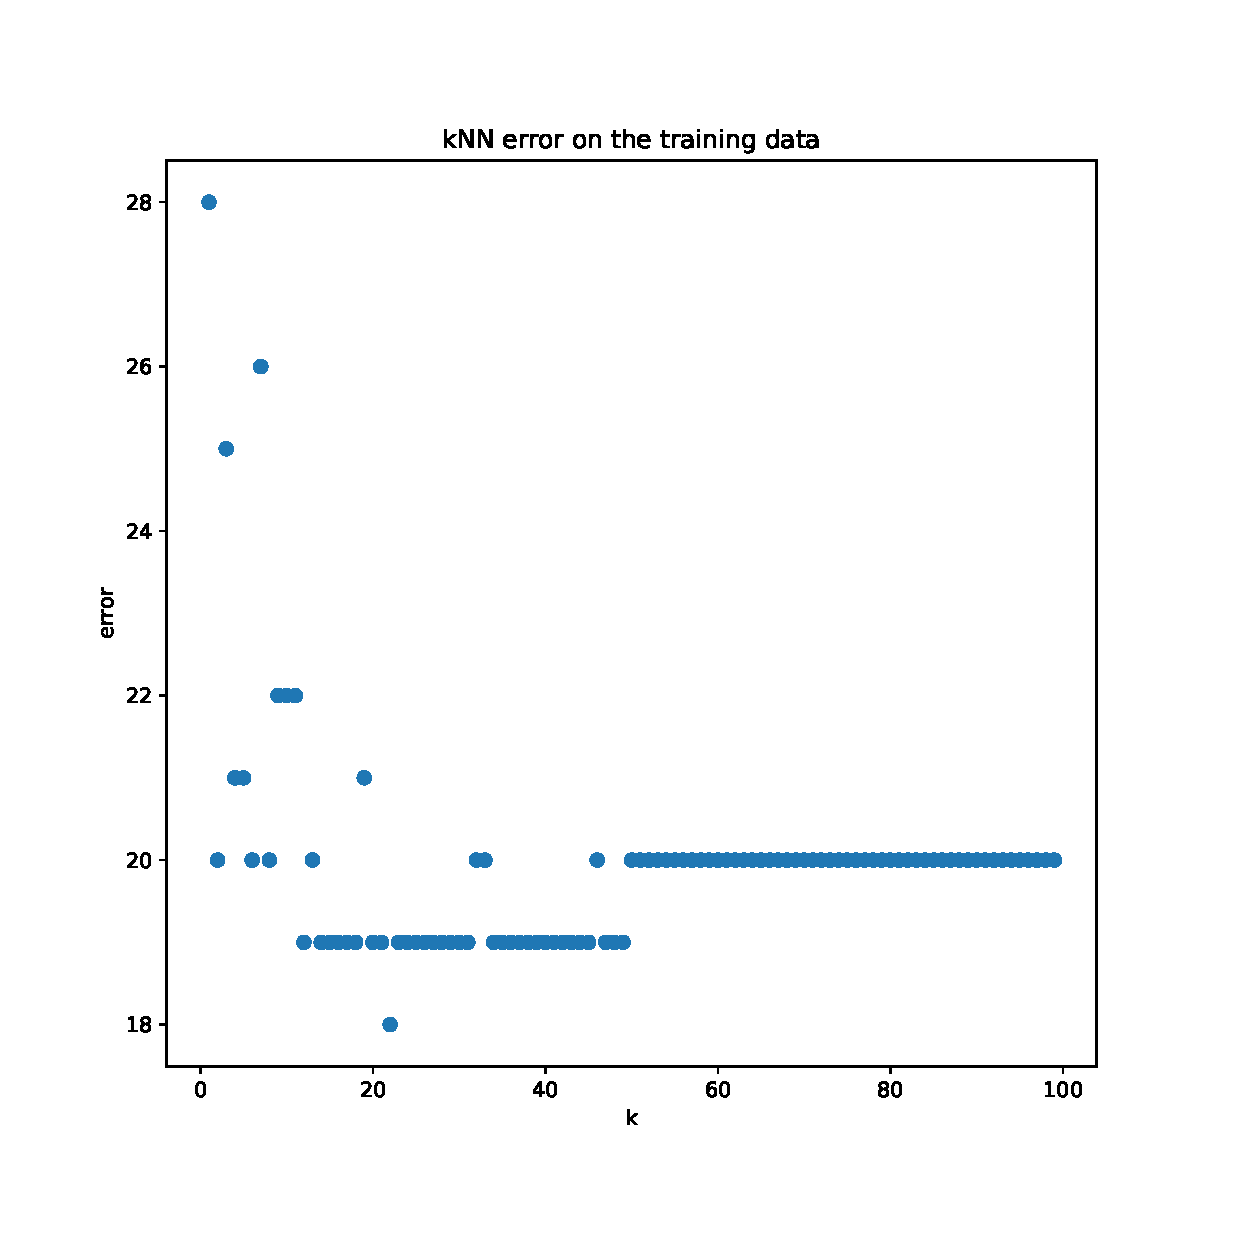
\includegraphics[width=\linewidth]{kNN-bin}
        \caption{kNN}
    \end{subfigure}%
    ~ 
    \begin{subfigure}[b]{0.5\textwidth}
        \centering
        \includegraphics[width=\linewidth]{pr_bin}
        \caption{Parzen-Rosenblatt window}
    \end{subfigure}
    \caption{Errors on the testing data for binary classification}
\end{figure*}


\begin{figure*}[t]
    \centering
    \begin{subfigure}[b]{0.5\textwidth}
        \centering
        \includegraphics[width=\linewidth]{kNN-mclass}
        \caption{kNN}
    \end{subfigure}%
    ~ 
    \begin{subfigure}[b]{0.5\textwidth}
        \centering
        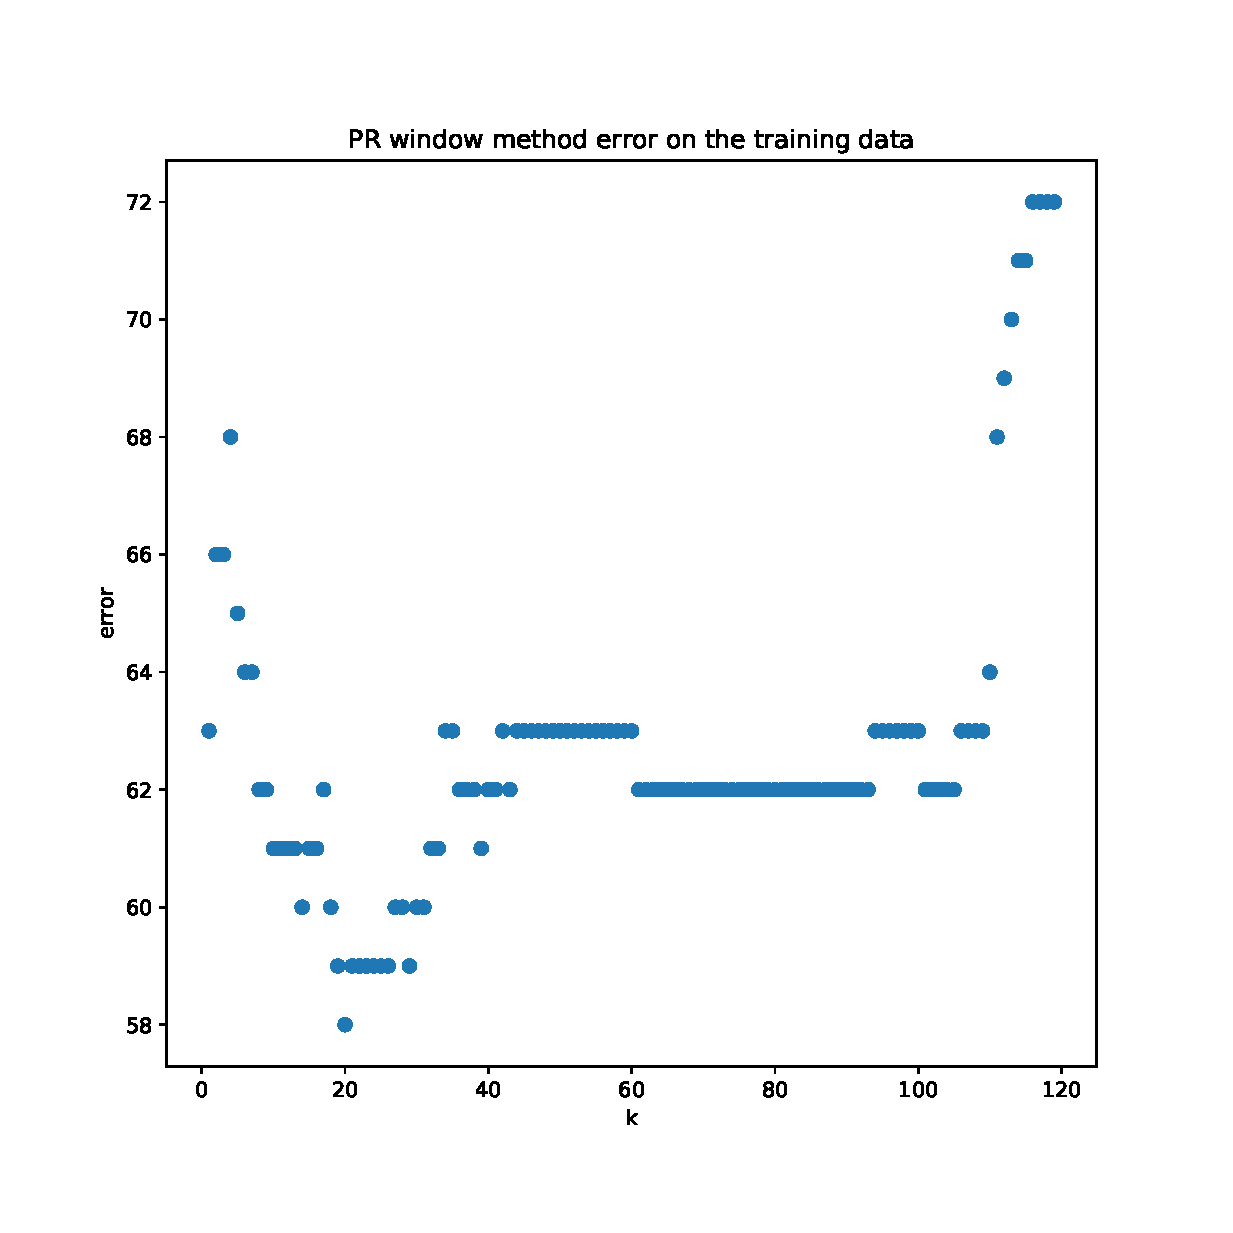
\includegraphics[width=\linewidth]{pr_mclass}
        \caption{Parzen-Rosenblatt window}
    \end{subfigure}
    \caption{Errors on the testing data for 3 class classification}
\end{figure*}

Best $k$ for binary classification turned out to be 22 (52 objects out of 70 are predicted correctly), for 3 classes this number is 11 (62 objects out of 120 are labeled correctly).

Parzen-Rosenblatt window method with chosen kernel has not shown a high accuracy in this problem. Best $k$ for binary classification is 3, but only 45 objects are predicted correctly. For the problem with 3 classes optimal $k$ is 20, 62 objects are predicted correctly.

As can be seen from figures for kNN, starting from specific $k$ error is not changing. It may happen because of big misbalance between numbers of elements in each class - starting from specific $k$ number of elements from dominating class always prevails. The second method does not have this issue.


\end{document}